% Options for packages loaded elsewhere
\PassOptionsToPackage{unicode}{hyperref}
\PassOptionsToPackage{hyphens}{url}
%
\documentclass[
  ignorenonframetext,
]{beamer}
\usepackage{pgfpages}
\setbeamertemplate{caption}[numbered]
\setbeamertemplate{caption label separator}{: }
\setbeamercolor{caption name}{fg=normal text.fg}
\beamertemplatenavigationsymbolsempty
% Prevent slide breaks in the middle of a paragraph
\widowpenalties 1 10000
\raggedbottom
\setbeamertemplate{part page}{
  \centering
  \begin{beamercolorbox}[sep=16pt,center]{part title}
    \usebeamerfont{part title}\insertpart\par
  \end{beamercolorbox}
}
\setbeamertemplate{section page}{
  \centering
  \begin{beamercolorbox}[sep=12pt,center]{part title}
    \usebeamerfont{section title}\insertsection\par
  \end{beamercolorbox}
}
\setbeamertemplate{subsection page}{
  \centering
  \begin{beamercolorbox}[sep=8pt,center]{part title}
    \usebeamerfont{subsection title}\insertsubsection\par
  \end{beamercolorbox}
}
\AtBeginPart{
  \frame{\partpage}
}
\AtBeginSection{
  \ifbibliography
  \else
    \frame{\sectionpage}
  \fi
}
\AtBeginSubsection{
  \frame{\subsectionpage}
}
\usepackage{lmodern}
\usepackage{amssymb,amsmath}
\usepackage{ifxetex,ifluatex}
\ifnum 0\ifxetex 1\fi\ifluatex 1\fi=0 % if pdftex
  \usepackage[T1]{fontenc}
  \usepackage[utf8]{inputenc}
  \usepackage{textcomp} % provide euro and other symbols
\else % if luatex or xetex
  \usepackage{unicode-math}
  \defaultfontfeatures{Scale=MatchLowercase}
  \defaultfontfeatures[\rmfamily]{Ligatures=TeX,Scale=1}
\fi
% Use upquote if available, for straight quotes in verbatim environments
\IfFileExists{upquote.sty}{\usepackage{upquote}}{}
\IfFileExists{microtype.sty}{% use microtype if available
  \usepackage[]{microtype}
  \UseMicrotypeSet[protrusion]{basicmath} % disable protrusion for tt fonts
}{}
\makeatletter
\@ifundefined{KOMAClassName}{% if non-KOMA class
  \IfFileExists{parskip.sty}{%
    \usepackage{parskip}
  }{% else
    \setlength{\parindent}{0pt}
    \setlength{\parskip}{6pt plus 2pt minus 1pt}}
}{% if KOMA class
  \KOMAoptions{parskip=half}}
\makeatother
\usepackage{xcolor}
\IfFileExists{xurl.sty}{\usepackage{xurl}}{} % add URL line breaks if available
\IfFileExists{bookmark.sty}{\usepackage{bookmark}}{\usepackage{hyperref}}
\hypersetup{
  pdftitle={Module 8: Bayesian Fellegi and Sunter},
  pdfauthor={Rebecca C. Steorts},
  hidelinks,
  pdfcreator={LaTeX via pandoc}}
\urlstyle{same} % disable monospaced font for URLs
\newif\ifbibliography
\usepackage{color}
\usepackage{fancyvrb}
\newcommand{\VerbBar}{|}
\newcommand{\VERB}{\Verb[commandchars=\\\{\}]}
\DefineVerbatimEnvironment{Highlighting}{Verbatim}{commandchars=\\\{\}}
% Add ',fontsize=\small' for more characters per line
\usepackage{framed}
\definecolor{shadecolor}{RGB}{248,248,248}
\newenvironment{Shaded}{\begin{snugshade}}{\end{snugshade}}
\newcommand{\AlertTok}[1]{\textcolor[rgb]{0.94,0.16,0.16}{#1}}
\newcommand{\AnnotationTok}[1]{\textcolor[rgb]{0.56,0.35,0.01}{\textbf{\textit{#1}}}}
\newcommand{\AttributeTok}[1]{\textcolor[rgb]{0.77,0.63,0.00}{#1}}
\newcommand{\BaseNTok}[1]{\textcolor[rgb]{0.00,0.00,0.81}{#1}}
\newcommand{\BuiltInTok}[1]{#1}
\newcommand{\CharTok}[1]{\textcolor[rgb]{0.31,0.60,0.02}{#1}}
\newcommand{\CommentTok}[1]{\textcolor[rgb]{0.56,0.35,0.01}{\textit{#1}}}
\newcommand{\CommentVarTok}[1]{\textcolor[rgb]{0.56,0.35,0.01}{\textbf{\textit{#1}}}}
\newcommand{\ConstantTok}[1]{\textcolor[rgb]{0.00,0.00,0.00}{#1}}
\newcommand{\ControlFlowTok}[1]{\textcolor[rgb]{0.13,0.29,0.53}{\textbf{#1}}}
\newcommand{\DataTypeTok}[1]{\textcolor[rgb]{0.13,0.29,0.53}{#1}}
\newcommand{\DecValTok}[1]{\textcolor[rgb]{0.00,0.00,0.81}{#1}}
\newcommand{\DocumentationTok}[1]{\textcolor[rgb]{0.56,0.35,0.01}{\textbf{\textit{#1}}}}
\newcommand{\ErrorTok}[1]{\textcolor[rgb]{0.64,0.00,0.00}{\textbf{#1}}}
\newcommand{\ExtensionTok}[1]{#1}
\newcommand{\FloatTok}[1]{\textcolor[rgb]{0.00,0.00,0.81}{#1}}
\newcommand{\FunctionTok}[1]{\textcolor[rgb]{0.00,0.00,0.00}{#1}}
\newcommand{\ImportTok}[1]{#1}
\newcommand{\InformationTok}[1]{\textcolor[rgb]{0.56,0.35,0.01}{\textbf{\textit{#1}}}}
\newcommand{\KeywordTok}[1]{\textcolor[rgb]{0.13,0.29,0.53}{\textbf{#1}}}
\newcommand{\NormalTok}[1]{#1}
\newcommand{\OperatorTok}[1]{\textcolor[rgb]{0.81,0.36,0.00}{\textbf{#1}}}
\newcommand{\OtherTok}[1]{\textcolor[rgb]{0.56,0.35,0.01}{#1}}
\newcommand{\PreprocessorTok}[1]{\textcolor[rgb]{0.56,0.35,0.01}{\textit{#1}}}
\newcommand{\RegionMarkerTok}[1]{#1}
\newcommand{\SpecialCharTok}[1]{\textcolor[rgb]{0.00,0.00,0.00}{#1}}
\newcommand{\SpecialStringTok}[1]{\textcolor[rgb]{0.31,0.60,0.02}{#1}}
\newcommand{\StringTok}[1]{\textcolor[rgb]{0.31,0.60,0.02}{#1}}
\newcommand{\VariableTok}[1]{\textcolor[rgb]{0.00,0.00,0.00}{#1}}
\newcommand{\VerbatimStringTok}[1]{\textcolor[rgb]{0.31,0.60,0.02}{#1}}
\newcommand{\WarningTok}[1]{\textcolor[rgb]{0.56,0.35,0.01}{\textbf{\textit{#1}}}}
\usepackage{graphicx,grffile}
\makeatletter
\def\maxwidth{\ifdim\Gin@nat@width>\linewidth\linewidth\else\Gin@nat@width\fi}
\def\maxheight{\ifdim\Gin@nat@height>\textheight\textheight\else\Gin@nat@height\fi}
\makeatother
% Scale images if necessary, so that they will not overflow the page
% margins by default, and it is still possible to overwrite the defaults
% using explicit options in \includegraphics[width, height, ...]{}
\setkeys{Gin}{width=\maxwidth,height=\maxheight,keepaspectratio}
% Set default figure placement to htbp
\makeatletter
\def\fps@figure{htbp}
\makeatother
\setlength{\emergencystretch}{3em} % prevent overfull lines
\providecommand{\tightlist}{%
  \setlength{\itemsep}{0pt}\setlength{\parskip}{0pt}}
\setcounter{secnumdepth}{-\maxdimen} % remove section numbering
% Custom definitions
% To use this customization file, insert the line "\input{custom}" in the header of the tex file.

% Formatting




% Packages

\usepackage{threeparttable,url}
\usepackage{animate}
\usepackage{dcolumn}
\usepackage{arydshln}
\usepackage{threeparttable}
\usepackage{etoolbox}
\usepackage{xmpmulti}
\usepackage{multirow}

\usepackage{tcolorbox}

\setbeamertemplate{navigation symbols}{}
\setbeamertemplate{footline}[page number]

 \usepackage{amssymb,latexsym}
\usepackage{amssymb,amsfonts,amsmath,latexsym,amsthm, bm}
%\usepackage[usenames,dvipsnames]{color}
%\usepackage[]{graphicx}
%\usepackage[space]{grffile}
\usepackage{mathrsfs}   % fancy math font
% \usepackage[font=small,skip=0pt]{caption}
%\usepackage[skip=0pt]{caption}
%\usepackage{subcaption}
%\usepackage{verbatim}
%\usepackage{url}
%\usepackage{bm}
\usepackage{dsfont}
\usepackage{multirow}
%\usepackage{extarrows}
%\usepackage{multirow}
%% \usepackage{wrapfig}
%% \usepackage{epstopdf}
%\usepackage{rotating}
%\usepackage{tikz}
%\usetikzlibrary{fit}					% fitting shapes to coordinates
%\usetikzlibrary{backgrounds}	% drawing the background after the foreground


% \usepackage[dvipdfm,colorlinks,citecolor=blue,linkcolor=blue,urlcolor=blue]{hyperref}
%\usepackage[colorlinks,citecolor=blue,linkcolor=blue,urlcolor=blue]{hyperref}
%%\usepackage{hyperref}
%\usepackage[authoryear,round]{natbib}


%  Theorems, etc.

%\theoremstyle{plain}
%\newtheorem{theorem}{Theorem}[section]
%\newtheorem{corollary}[theorem]{Corollary}
%\newtheorem{lemma}[theorem]{Lemma}
%\newtheorem{proposition}[theorem]{Proposition}
%\newtheorem{condition}[theorem]{Condition}
% \newtheorem{conditions}[theorem]{Conditions}

%\theoremstyle{definition}
%\newtheorem{definition}[theorem]{Definition}
%% \newtheorem*{unnumbered-definition}{Definition}
%\newtheorem{example}[theorem]{Example}
%\theoremstyle{remark}
%\newtheorem*{remark}{Remark}
%\numberwithin{equation}{section}




% Document-specific shortcuts
\newcommand{\btheta}{{\bm\theta}}
\newcommand{\bbtheta}{{\pmb{\bm\theta}}}

\newcommand{\commentary}[1]{\ifx\showcommentary\undefined\else \emph{#1}\fi}

\newcommand{\term}[1]{\textit{\textbf{#1}}}

% Math shortcuts

% Probability distributions
\DeclareMathOperator*{\Exp}{Exp}
\DeclareMathOperator*{\TExp}{TExp}
\DeclareMathOperator*{\Bernoulli}{Bernoulli}
\DeclareMathOperator*{\Beta}{Beta}
\DeclareMathOperator*{\Ga}{Gamma}
\DeclareMathOperator*{\TGamma}{TGamma}
\DeclareMathOperator*{\Poisson}{Poisson}
\DeclareMathOperator*{\Binomial}{Binomial}
\DeclareMathOperator*{\NormalGamma}{NormalGamma}
\DeclareMathOperator*{\InvGamma}{InvGamma}
\DeclareMathOperator*{\Cauchy}{Cauchy}
\DeclareMathOperator*{\Uniform}{Uniform}
\DeclareMathOperator*{\Gumbel}{Gumbel}
\DeclareMathOperator*{\Pareto}{Pareto}
\DeclareMathOperator*{\Mono}{Mono}
\DeclareMathOperator*{\Geometric}{Geometric}
\DeclareMathOperator*{\Wishart}{Wishart}

% Math operators
\DeclareMathOperator*{\argmin}{arg\,min}
\DeclareMathOperator*{\argmax}{arg\,max}
\DeclareMathOperator*{\Cov}{Cov}
\DeclareMathOperator*{\diag}{diag}
\DeclareMathOperator*{\median}{median}
\DeclareMathOperator*{\Vol}{Vol}

% Math characters
\newcommand{\R}{\mathbb{R}}
\newcommand{\Z}{\mathbb{Z}}
\newcommand{\E}{\mathbb{E}}
\renewcommand{\Pr}{\mathbb{P}}
\newcommand{\I}{\mathds{1}}
\newcommand{\V}{\mathbb{V}}

\newcommand{\A}{\mathcal{A}}
%\newcommand{\C}{\mathcal{C}}
\newcommand{\D}{\mathcal{D}}
\newcommand{\Hcal}{\mathcal{H}}
\newcommand{\M}{\mathcal{M}}
\newcommand{\N}{\mathcal{N}}
\newcommand{\X}{\mathcal{X}}
\newcommand{\Zcal}{\mathcal{Z}}
\renewcommand{\P}{\mathcal{P}}

\newcommand{\T}{\mathtt{T}}
\renewcommand{\emptyset}{\varnothing}


% Miscellaneous commands
\newcommand{\iid}{\stackrel{\mathrm{iid}}{\sim}}
\newcommand{\matrixsmall}[1]{\bigl(\begin{smallmatrix}#1\end{smallmatrix} \bigr)}

\newcommand{\items}[1]{\begin{itemize} #1 \end{itemize}}

\newcommand{\todo}[1]{\emph{\textcolor{red}{(#1)}}}

\newcommand{\branch}[4]{
\left\{
	\begin{array}{ll}
		#1  & \mbox{if } #2 \\
		#3 & \mbox{if } #4
	\end{array}
\right.
}

% approximately proportional to
\def\app#1#2{%
  \mathrel{%
    \setbox0=\hbox{$#1\sim$}%
    \setbox2=\hbox{%
      \rlap{\hbox{$#1\propto$}}%
      \lower1.3\ht0\box0%
    }%
    \raise0.25\ht2\box2%
  }%
}
\def\approxprop{\mathpalette\app\relax}

% \newcommand{\approptoinn}[2]{\mathrel{\vcenter{
  % \offinterlineskip\halign{\hfil$##$\cr
    % #1\propto\cr\noalign{\kern2pt}#1\sim\cr\noalign{\kern-2pt}}}}}

% \newcommand{\approxpropto}{\mathpalette\approptoinn\relax}

\title{Module 8: Bayesian Fellegi and Sunter}
\author{Rebecca C. Steorts}
\date{}

\begin{document}
\frame{\titlepage}

\begin{frame}{BDD package}
\protect\hypertarget{bdd-package}{}

\begin{itemize}
\tightlist
\item
  Marchant, Rubinstein, and Steorts (2021) have provided a package for
  implementing Sadinle (2014), which is referred to as BDD (Bayesian
  Duplicated Detection).
\end{itemize}

\end{frame}

\begin{frame}[fragile]{RLdata500 data set}
\protect\hypertarget{rldata500-data-set}{}

\begin{itemize}
\tightlist
\item
  We investigate it on the RLdata500 data set.
\end{itemize}

\footnotesize

\begin{Shaded}
\begin{Highlighting}[]
\KeywordTok{library}\NormalTok{(magrittr)    }\CommentTok{# pipe operator (must be loaded before BDD)}
\KeywordTok{library}\NormalTok{(comparator)  }\CommentTok{# normalized Levenshtein distance}
\KeywordTok{library}\NormalTok{(clevr)       }\CommentTok{# evaluation functions}
\KeywordTok{library}\NormalTok{(BDD)}
\NormalTok{RLdata500[[}\StringTok{'rec_id'}\NormalTok{]] <-}\StringTok{ }\KeywordTok{seq.int}\NormalTok{(}\DataTypeTok{length.out=}\KeywordTok{nrow}\NormalTok{(RLdata500))}
\KeywordTok{head}\NormalTok{(RLdata500)}
\end{Highlighting}
\end{Shaded}

\begin{verbatim}
##   fname_c1 fname_c2 lname_c1 lname_c2   by bm bd rec_id
## 1  CARSTEN     <NA>    MEIER     <NA> 1949  7 22      1
## 2     GERD     <NA>    BAUER     <NA> 1968  7 27      2
## 3   ROBERT     <NA> HARTMANN     <NA> 1930  4 30      3
## 4   STEFAN     <NA>    WOLFF     <NA> 1957  9  2      4
## 5     RALF     <NA>  KRUEGER     <NA> 1966  1 13      5
## 6  JUERGEN     <NA>   FRANKE     <NA> 1929  7  4      6
\end{verbatim}

\end{frame}

\begin{frame}[fragile]{Distance functions}
\protect\hypertarget{distance-functions}{}

\begin{Shaded}
\begin{Highlighting}[]
\NormalTok{scoring_fns <-}\StringTok{ }\KeywordTok{list}\NormalTok{(}
  \DataTypeTok{fname_c1 =} \KeywordTok{Levenshtein}\NormalTok{(}\DataTypeTok{normalize =} \OtherTok{TRUE}\NormalTok{),}
  \DataTypeTok{lname_c1 =} \KeywordTok{Levenshtein}\NormalTok{(}\DataTypeTok{normalize =} \OtherTok{TRUE}\NormalTok{),}
  \DataTypeTok{by =} \ControlFlowTok{function}\NormalTok{(x, y) }\KeywordTok{abs}\NormalTok{(x }\OperatorTok{-}\StringTok{ }\NormalTok{y),}
  \DataTypeTok{bm =} \ControlFlowTok{function}\NormalTok{(x, y) }\KeywordTok{abs}\NormalTok{(x }\OperatorTok{-}\StringTok{ }\NormalTok{y),}
  \DataTypeTok{bd =} \ControlFlowTok{function}\NormalTok{(x, y) }\KeywordTok{abs}\NormalTok{(x }\OperatorTok{-}\StringTok{ }\NormalTok{y)}
\NormalTok{)}
\end{Highlighting}
\end{Shaded}

\end{frame}

\begin{frame}[fragile]{Breaks}
\protect\hypertarget{breaks}{}

For each scoring function above, we provide a breaks vectors, which
specifies the discrete levels of agreement (from `high' agreement to
`low').

\begin{Shaded}
\begin{Highlighting}[]
\NormalTok{scoring_breaks <-}\StringTok{ }\KeywordTok{list}\NormalTok{(}
  \DataTypeTok{fname_c1 =} \KeywordTok{c}\NormalTok{(}\OperatorTok{-}\OtherTok{Inf}\NormalTok{,.}\DecValTok{05}\NormalTok{,.}\DecValTok{15}\NormalTok{,.}\DecValTok{3}\NormalTok{,}\OtherTok{Inf}\NormalTok{),}
  \DataTypeTok{lname_c1 =} \KeywordTok{c}\NormalTok{(}\OperatorTok{-}\OtherTok{Inf}\NormalTok{,.}\DecValTok{05}\NormalTok{,.}\DecValTok{15}\NormalTok{,.}\DecValTok{3}\NormalTok{,}\OtherTok{Inf}\NormalTok{),}
  \DataTypeTok{by =} \KeywordTok{c}\NormalTok{(}\OperatorTok{-}\OtherTok{Inf}\NormalTok{,}\DecValTok{0}\NormalTok{,}\DecValTok{1}\NormalTok{,}\DecValTok{3}\NormalTok{,}\OtherTok{Inf}\NormalTok{),}
  \DataTypeTok{bm =} \KeywordTok{c}\NormalTok{(}\OperatorTok{-}\OtherTok{Inf}\NormalTok{,}\DecValTok{0}\NormalTok{,}\DecValTok{1}\NormalTok{,}\DecValTok{3}\NormalTok{,}\OtherTok{Inf}\NormalTok{),}
  \DataTypeTok{bd =} \KeywordTok{c}\NormalTok{(}\OperatorTok{-}\OtherTok{Inf}\NormalTok{,}\DecValTok{0}\NormalTok{,}\DecValTok{2}\NormalTok{,}\DecValTok{7}\NormalTok{,}\OtherTok{Inf}\NormalTok{)}
\NormalTok{)}
\end{Highlighting}
\end{Shaded}

\end{frame}

\begin{frame}[fragile]{Comparison vectors}
\protect\hypertarget{comparison-vectors}{}

\begin{itemize}
\item
  Now we are ready to compute the attribute comparison scores for the
  record pairs.
\item
  Since this is a small data set, we consider all pairs using the
  \texttt{pairs\_all} function.
\item
  For larger data sets, blocking/indexing is recommended using
  \texttt{pairs\_hamming}, \texttt{pairs\_fuzzyblock}, or a custom
  blocking function.
\end{itemize}

\end{frame}

\begin{frame}[fragile]{Comparison vectors}
\protect\hypertarget{comparison-vectors-1}{}

\begin{Shaded}
\begin{Highlighting}[]
\NormalTok{pairs <-}\StringTok{ }\KeywordTok{pairs_all}\NormalTok{(RLdata500}\OperatorTok{$}\NormalTok{rec_id) }\OperatorTok
\StringTok{  }\KeywordTok{compute_scores}\NormalTok{(RLdata500, scoring_fns, }\DataTypeTok{id_col =} \StringTok{'rec_id'}\NormalTok{) }\OperatorTok\StringTok{ }
\StringTok{  }\KeywordTok{discretize_scores}\NormalTok{(scoring_breaks)}
\end{Highlighting}
\end{Shaded}

\end{frame}

\begin{frame}{Speeding up inference}
\protect\hypertarget{speeding-up-inference}{}

\begin{itemize}
\item
  To speed up inference, we only consider a subset of the pairs as
  candidate matches.
\item
  Specifically, we consider pairs that have a strong agreement on name
  (accounting for missing names).
\end{itemize}

\end{frame}

\begin{frame}[fragile]{Speeding up inference}
\protect\hypertarget{speeding-up-inference-1}{}

To speed up inference, we only consider a subset of the pairs as
candidate matches.

Specifically, we consider pairs that have a strong agreement on name
(accounting for missing names).

\vspace*{1em}

\tiny

\begin{Shaded}
\begin{Highlighting}[]
\NormalTok{pairs[[}\StringTok{'candidate'}\NormalTok{]] <-}\StringTok{ }\NormalTok{(pairs}\OperatorTok{$}\NormalTok{fname_c1 }\OperatorTok{<}\StringTok{ }\DecValTok{4}\NormalTok{) }\OperatorTok{&}\StringTok{ }\NormalTok{(pairs}\OperatorTok{$}\NormalTok{lname_c1 }\OperatorTok{<}\StringTok{ }\DecValTok{4}\NormalTok{) }\OperatorTok{|}\StringTok{ }
\StringTok{                            }\KeywordTok{is.na}\NormalTok{(pairs}\OperatorTok{$}\NormalTok{fname_c1) }\OperatorTok{|}\StringTok{ }\KeywordTok{is.na}\NormalTok{(pairs}\OperatorTok{$}\NormalTok{lname_c1) }
\end{Highlighting}
\end{Shaded}

\end{frame}

\begin{frame}[fragile]{priors on \(m\) and \(u\) probabilities}
\protect\hypertarget{priors-on-m-and-u-probabilities}{}

\begin{itemize}
\item
  Next we specify the priors on the m* and u* probabilities for each
  attribute and agreement level.
\item
  \texttt{lambda} contains the lower truncation points for the truncated
  Beta priors on the m* probabilities. \texttt{alpha1} and
  \texttt{beta1} are the shape parameters for the truncated Beta
  distributions to the \texttt{BDD} function below.
\item
  The Beta priors on the u* probabilities are uniform by default but can
  be adjusted using the alpha0 and beta0 arguments.
\end{itemize}

\end{frame}

\begin{frame}[fragile]{priors on \(m\) and \(u\) probabilities}
\protect\hypertarget{priors-on-m-and-u-probabilities-1}{}

\begin{Shaded}
\begin{Highlighting}[]
\NormalTok{lambda <-}\StringTok{ }\KeywordTok{list}\NormalTok{(}
  \DataTypeTok{fname_c1 =} \KeywordTok{c}\NormalTok{(}\FloatTok{0.8}\NormalTok{,}\FloatTok{0.85}\NormalTok{,}\FloatTok{0.99}\NormalTok{),}
  \DataTypeTok{lname_c1 =} \KeywordTok{c}\NormalTok{(}\FloatTok{0.8}\NormalTok{,}\FloatTok{0.85}\NormalTok{,}\FloatTok{0.99}\NormalTok{),}
  \DataTypeTok{by =} \KeywordTok{c}\NormalTok{(}\FloatTok{0.8}\NormalTok{,}\FloatTok{0.85}\NormalTok{,}\FloatTok{0.99}\NormalTok{),}
  \DataTypeTok{bm =} \KeywordTok{c}\NormalTok{(}\FloatTok{0.8}\NormalTok{,}\FloatTok{0.85}\NormalTok{,}\FloatTok{0.99}\NormalTok{),}
  \DataTypeTok{bd =} \KeywordTok{c}\NormalTok{(}\FloatTok{0.8}\NormalTok{,}\FloatTok{0.85}\NormalTok{,}\FloatTok{0.99}\NormalTok{)}
\NormalTok{)}
\end{Highlighting}
\end{Shaded}

\end{frame}

\begin{frame}[fragile]{Intialization and Gibbs sampler}
\protect\hypertarget{intialization-and-gibbs-sampler}{}

Finally we initialize the model and run inference using Markov chain
Monte Carlo.

\begin{Shaded}
\begin{Highlighting}[]
\NormalTok{model <-}\StringTok{ }\KeywordTok{BDD}\NormalTok{(pairs, lambda, }
             \DataTypeTok{id_cols =} \KeywordTok{c}\NormalTok{(}\StringTok{"rec_id.x"}\NormalTok{, }\StringTok{"rec_id.y"}\NormalTok{), }
             \DataTypeTok{candidate_col =} \StringTok{"candidate"}\NormalTok{)}
\NormalTok{fit <-}\StringTok{ }\KeywordTok{run_inference}\NormalTok{(model, }\DecValTok{100}\NormalTok{, }
                     \DataTypeTok{thin_interval =} \DecValTok{10}\NormalTok{, }
                     \DataTypeTok{burnin_interval =} \DecValTok{100}\NormalTok{)}
\CommentTok{# Completed sampling in 0.7 seconds}
\end{Highlighting}
\end{Shaded}

\end{frame}

\begin{frame}[fragile]{Posterior samples}
\protect\hypertarget{posterior-samples}{}

\begin{itemize}
\item
  The posterior samples of the linkage structure can be accessed by
  calling \texttt{extract(fit,\ "links")}.
\item
  However, these samples only cover the records that were considered as
  candidate pairs.
\item
  We can obtain samples of the complete linkage structure (for all
  records) using the following function.
\end{itemize}

\begin{Shaded}
\begin{Highlighting}[]
\NormalTok{links_samples <-}\StringTok{ }
\StringTok{  }\KeywordTok{complete_links_samples}\NormalTok{(fit, RLdata500}\OperatorTok{$}\NormalTok{rec_id)}
\end{Highlighting}
\end{Shaded}

\end{frame}

\begin{frame}{Traceplot of the cluster sizes}
\protect\hypertarget{traceplot-of-the-cluster-sizes}{}

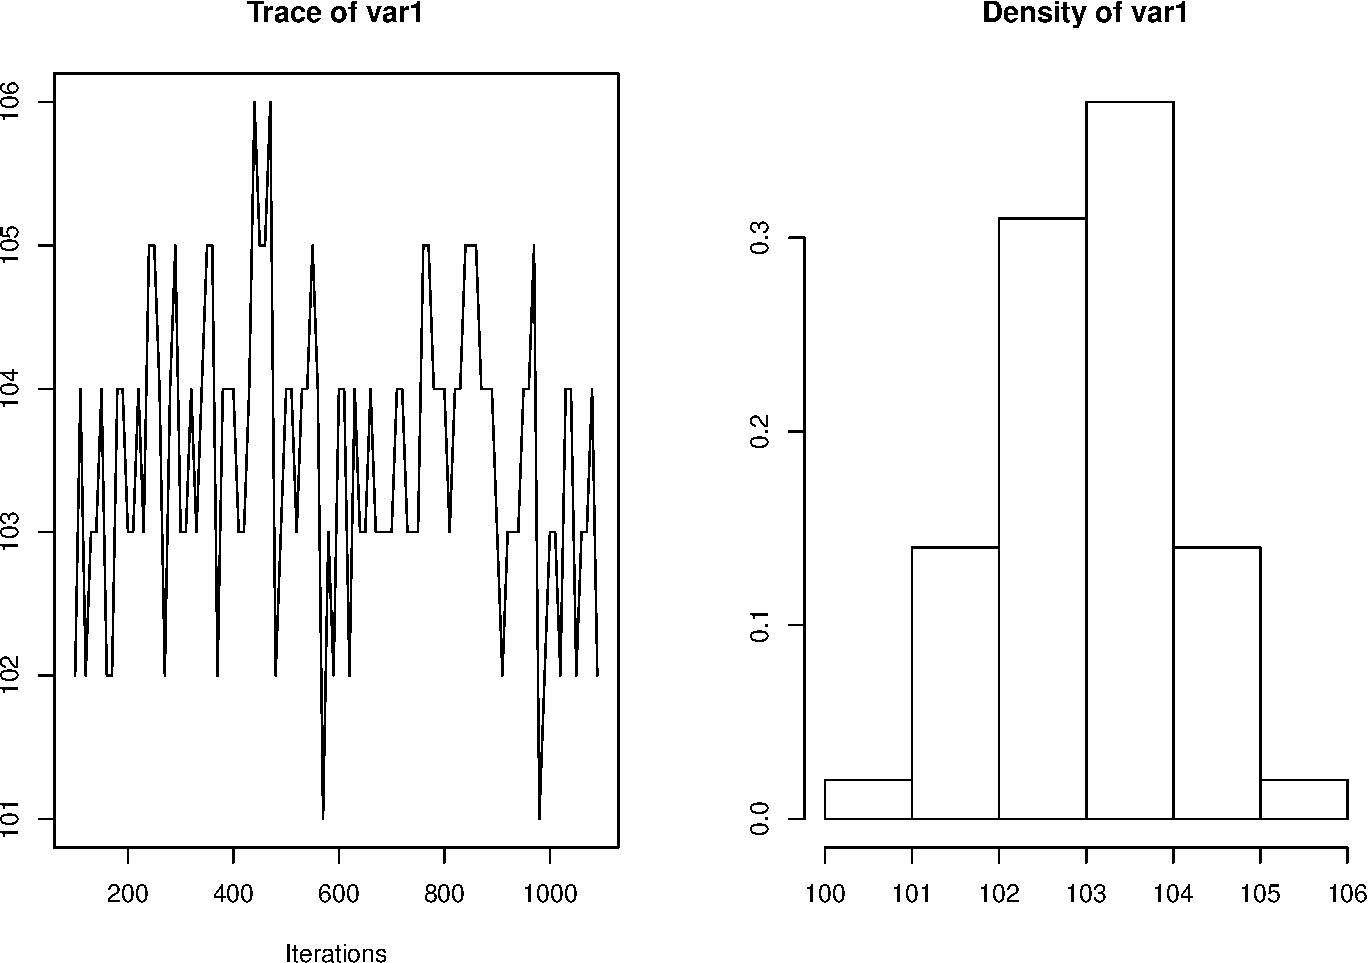
\includegraphics{bayesian-fellegi-sunter-vignette_files/figure-beamer/unnamed-chunk-9-1.pdf}

\end{frame}

\begin{frame}{Traceplot of the m probabilities}
\protect\hypertarget{traceplot-of-the-m-probabilities}{}

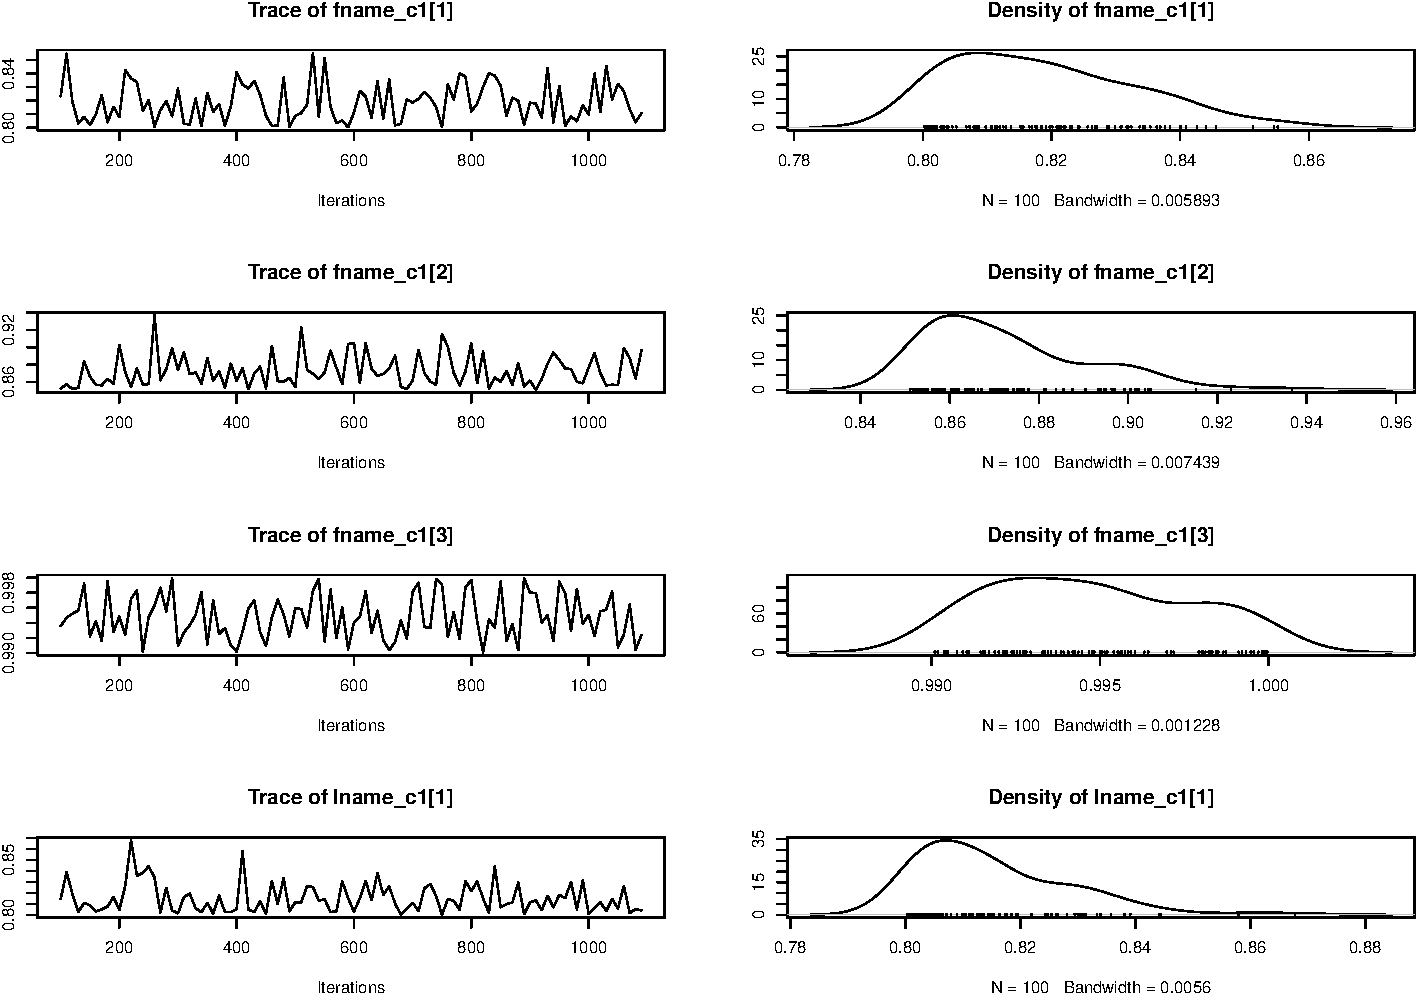
\includegraphics{bayesian-fellegi-sunter-vignette_files/figure-beamer/unnamed-chunk-10-1.pdf}
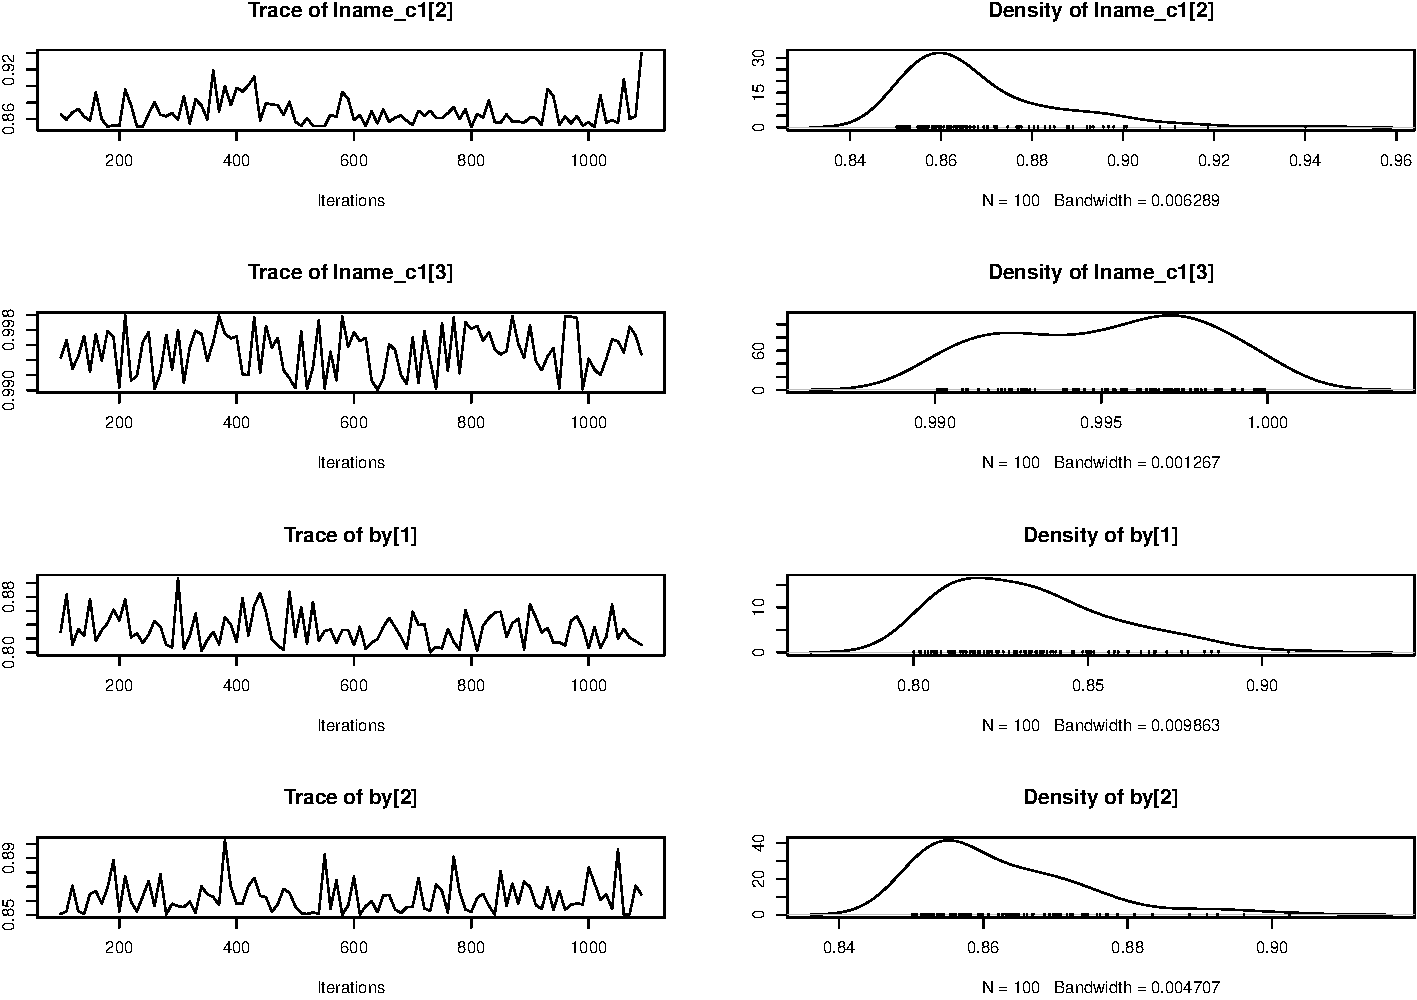
\includegraphics{bayesian-fellegi-sunter-vignette_files/figure-beamer/unnamed-chunk-10-2.pdf}
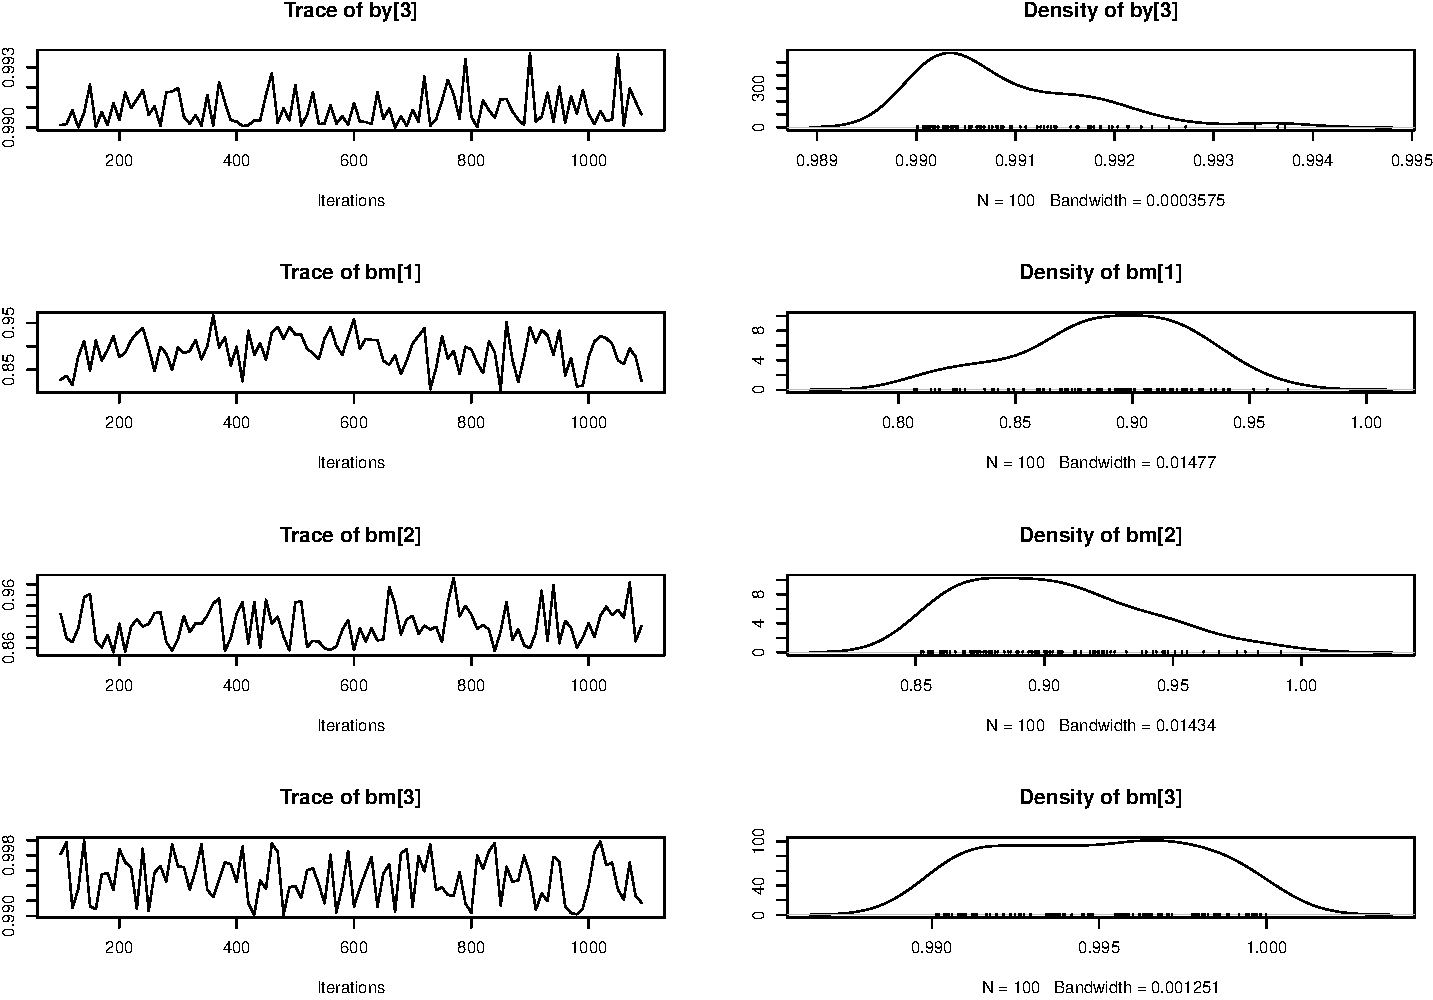
\includegraphics{bayesian-fellegi-sunter-vignette_files/figure-beamer/unnamed-chunk-10-3.pdf}
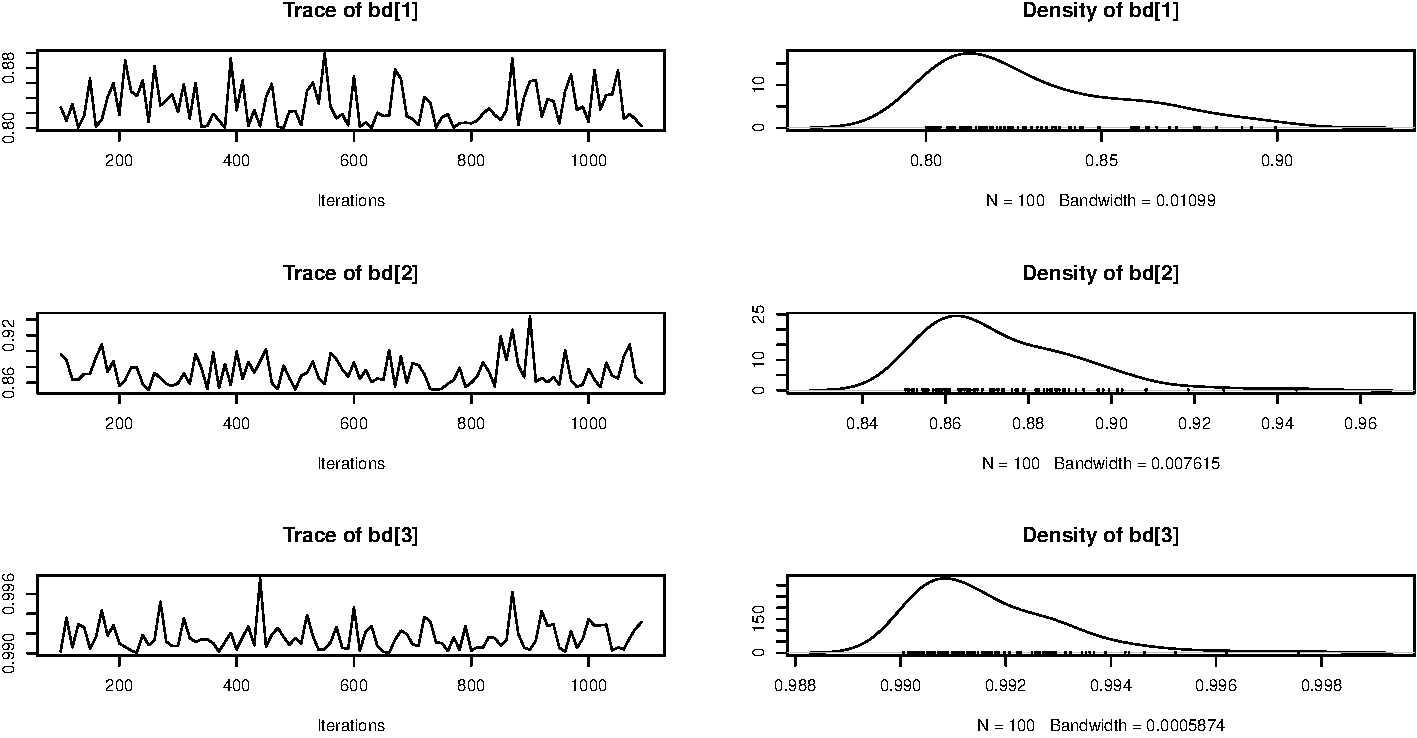
\includegraphics{bayesian-fellegi-sunter-vignette_files/figure-beamer/unnamed-chunk-10-4.pdf}

\end{frame}

\begin{frame}{Traceplot of the u probabilities}
\protect\hypertarget{traceplot-of-the-u-probabilities}{}

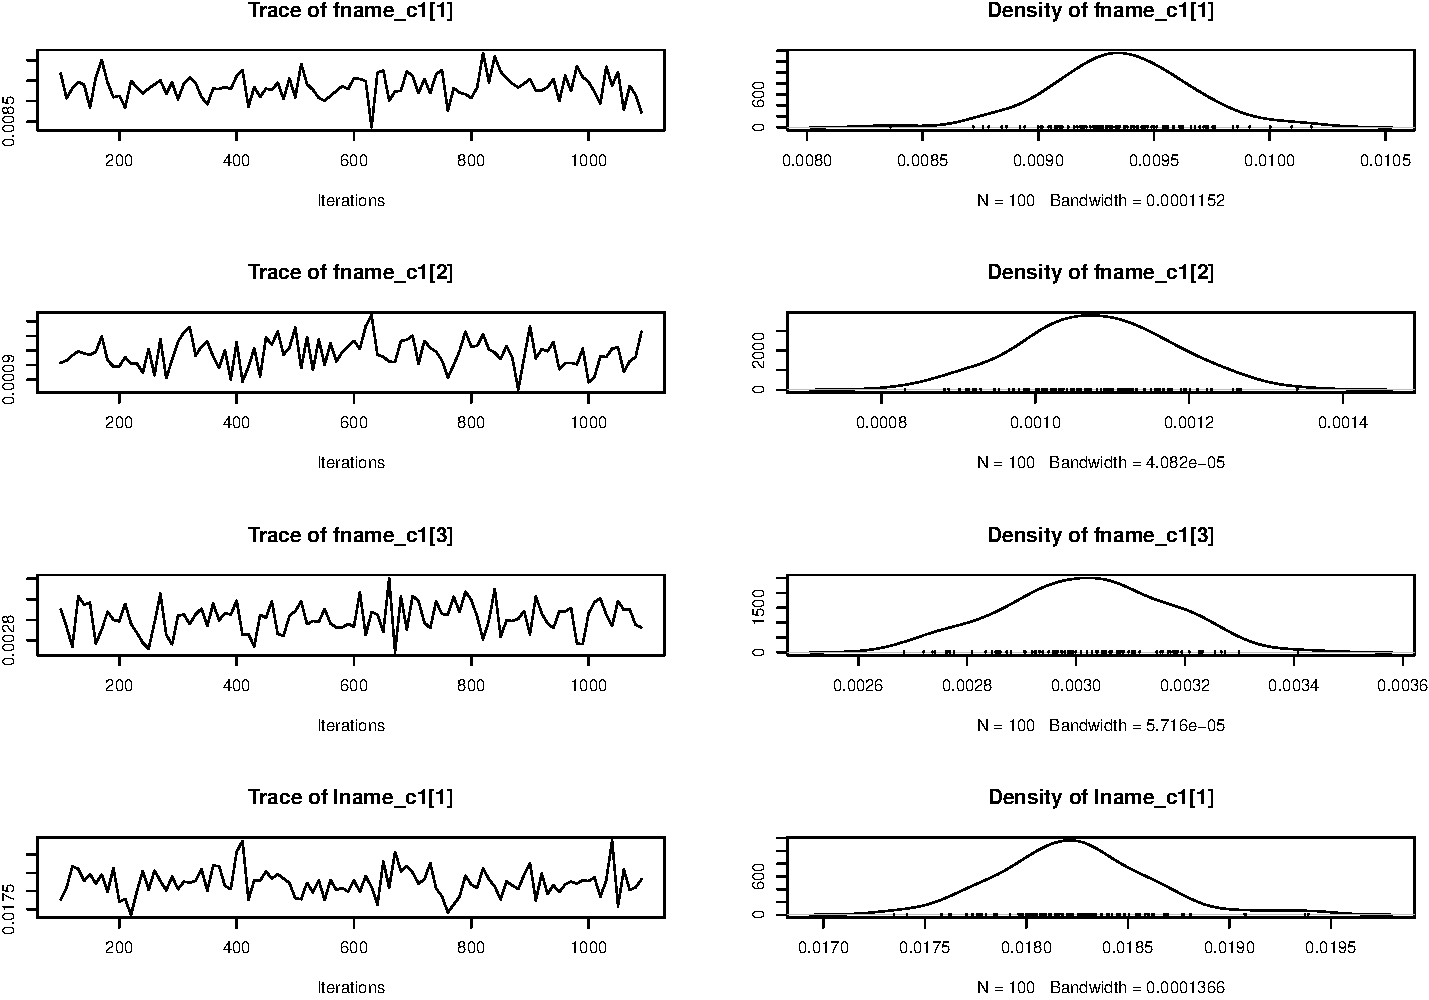
\includegraphics{bayesian-fellegi-sunter-vignette_files/figure-beamer/unnamed-chunk-11-1.pdf}
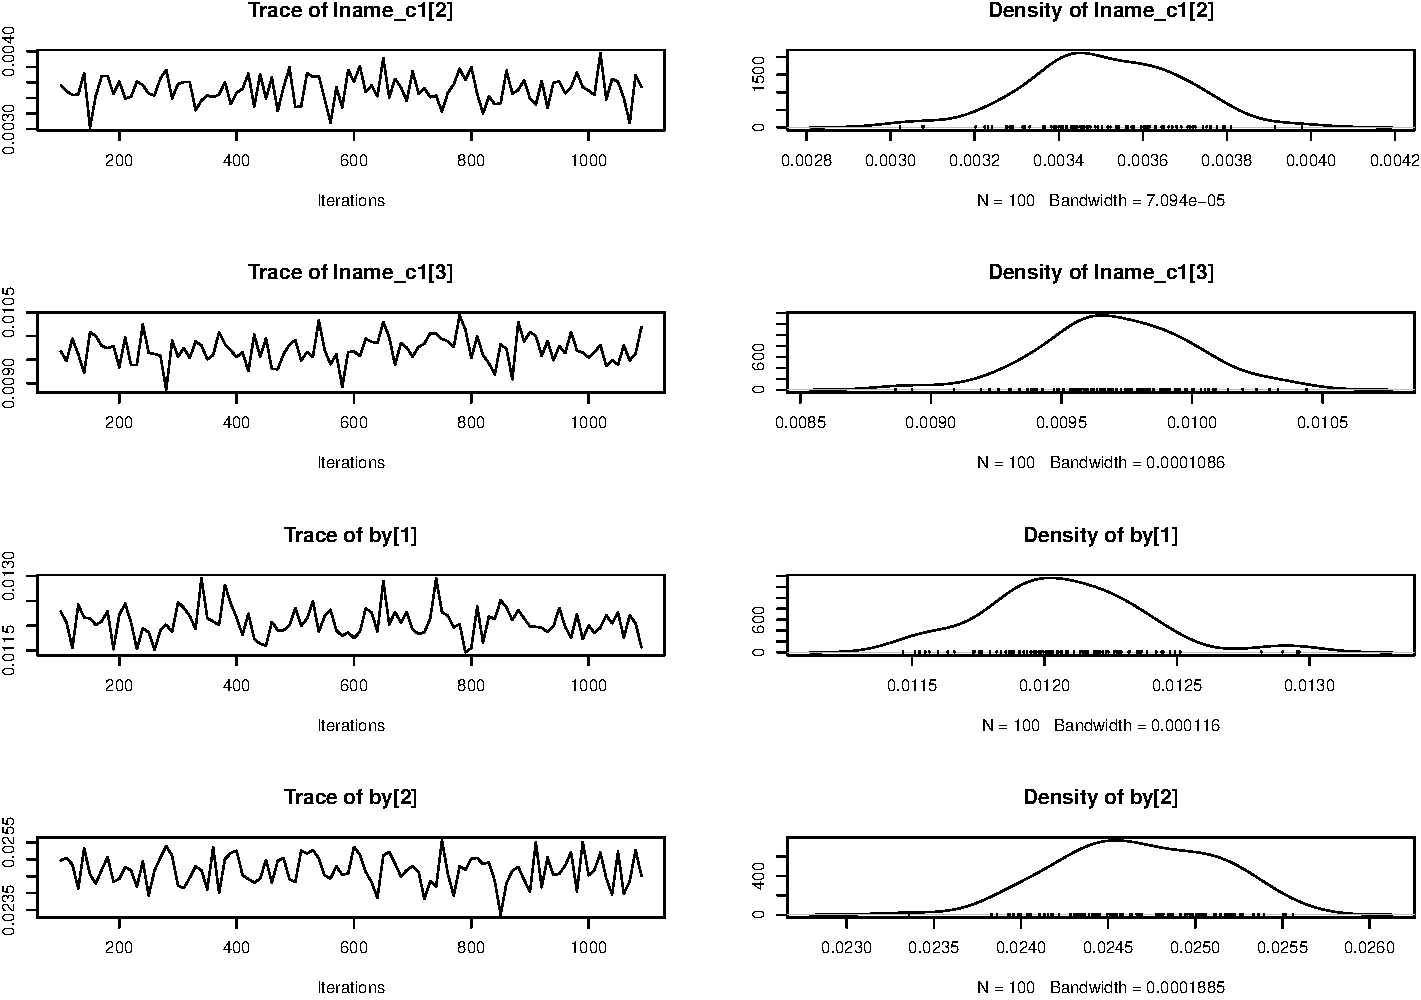
\includegraphics{bayesian-fellegi-sunter-vignette_files/figure-beamer/unnamed-chunk-11-2.pdf}
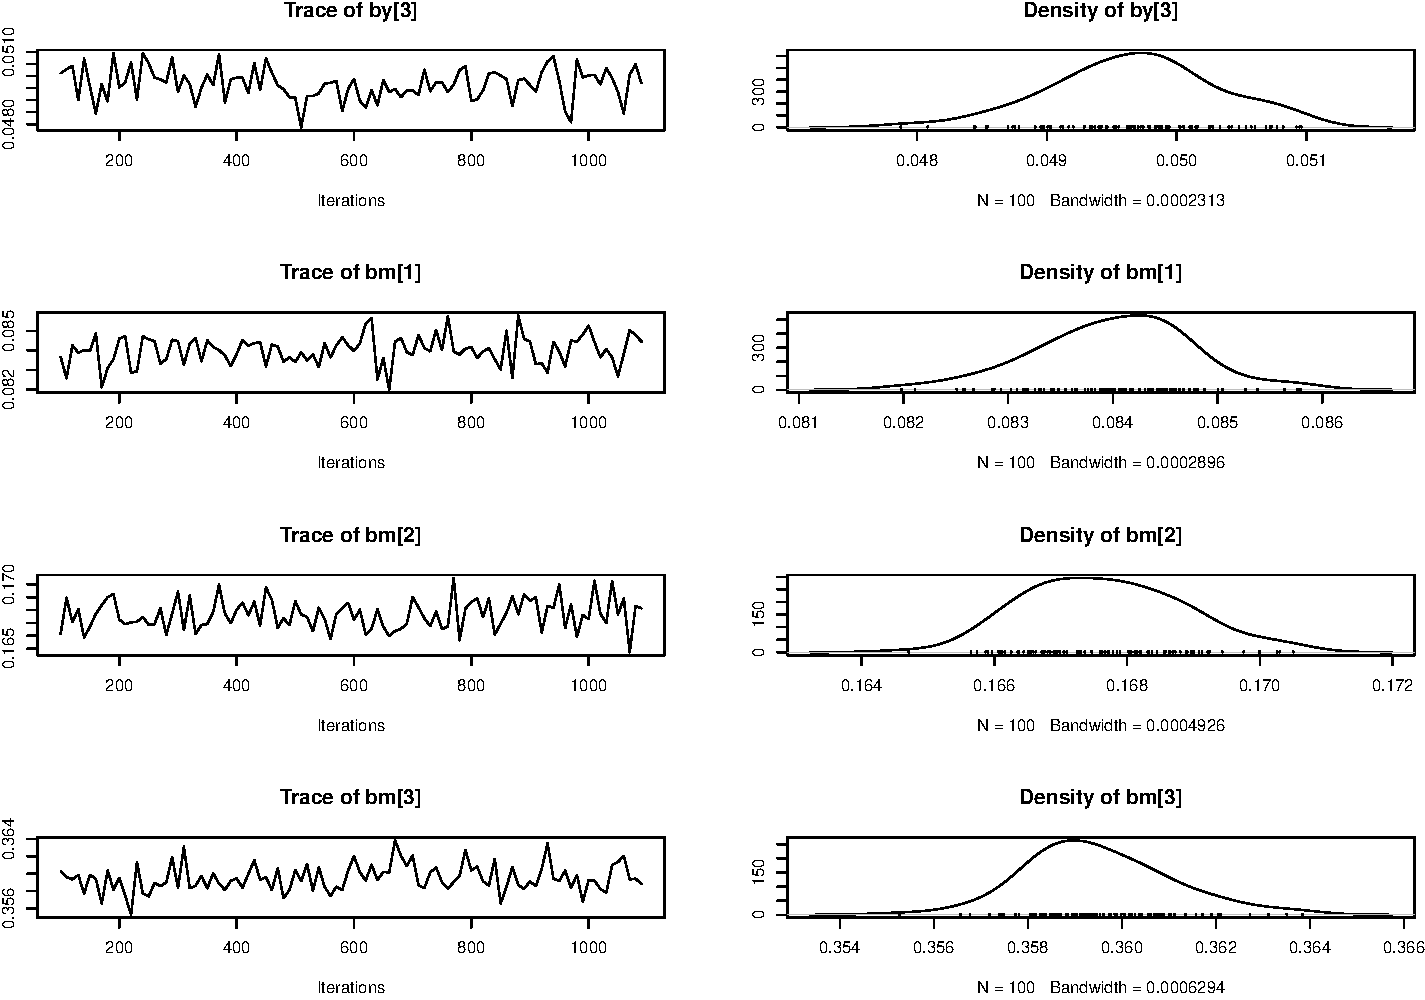
\includegraphics{bayesian-fellegi-sunter-vignette_files/figure-beamer/unnamed-chunk-11-3.pdf}
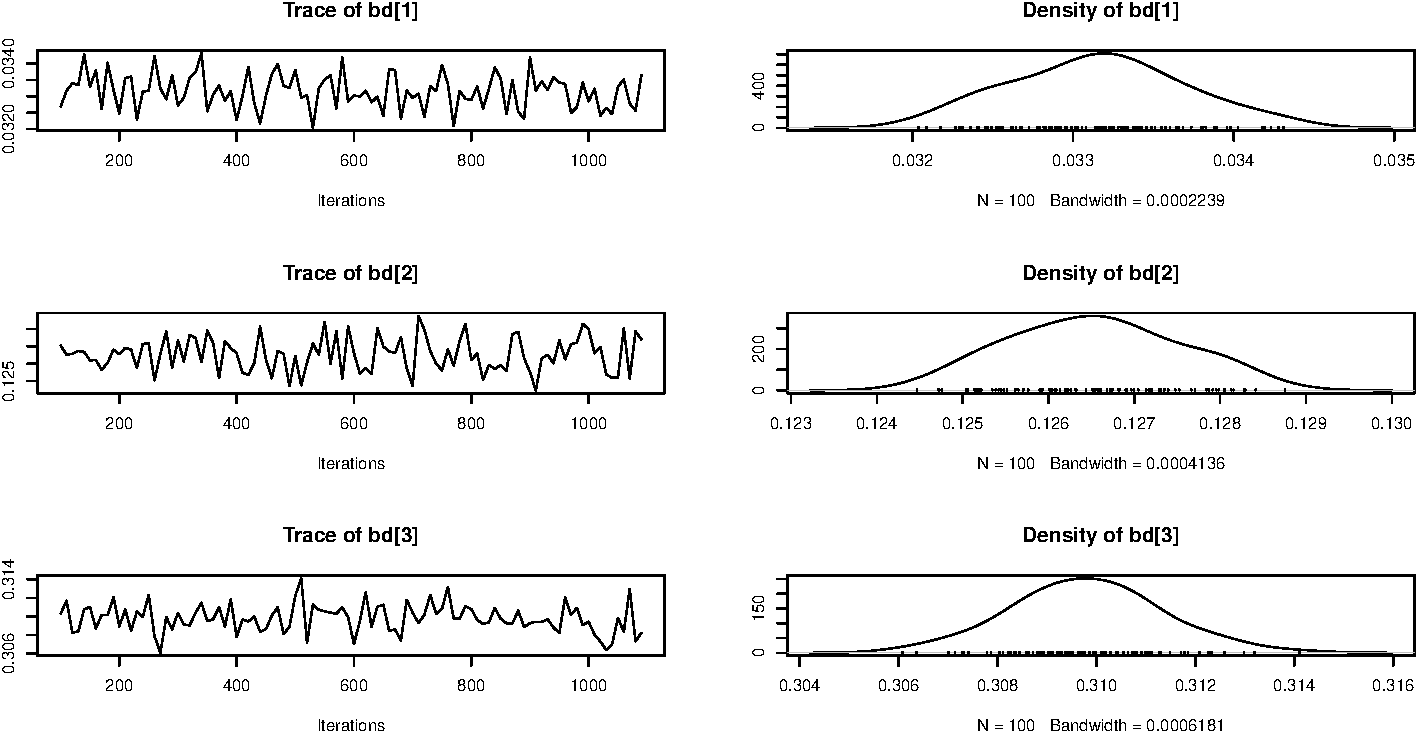
\includegraphics{bayesian-fellegi-sunter-vignette_files/figure-beamer/unnamed-chunk-11-4.pdf}

\end{frame}

\begin{frame}{Pairwise Evaluation Metrics (Boxplots)}
\protect\hypertarget{pairwise-evaluation-metrics-boxplots}{}

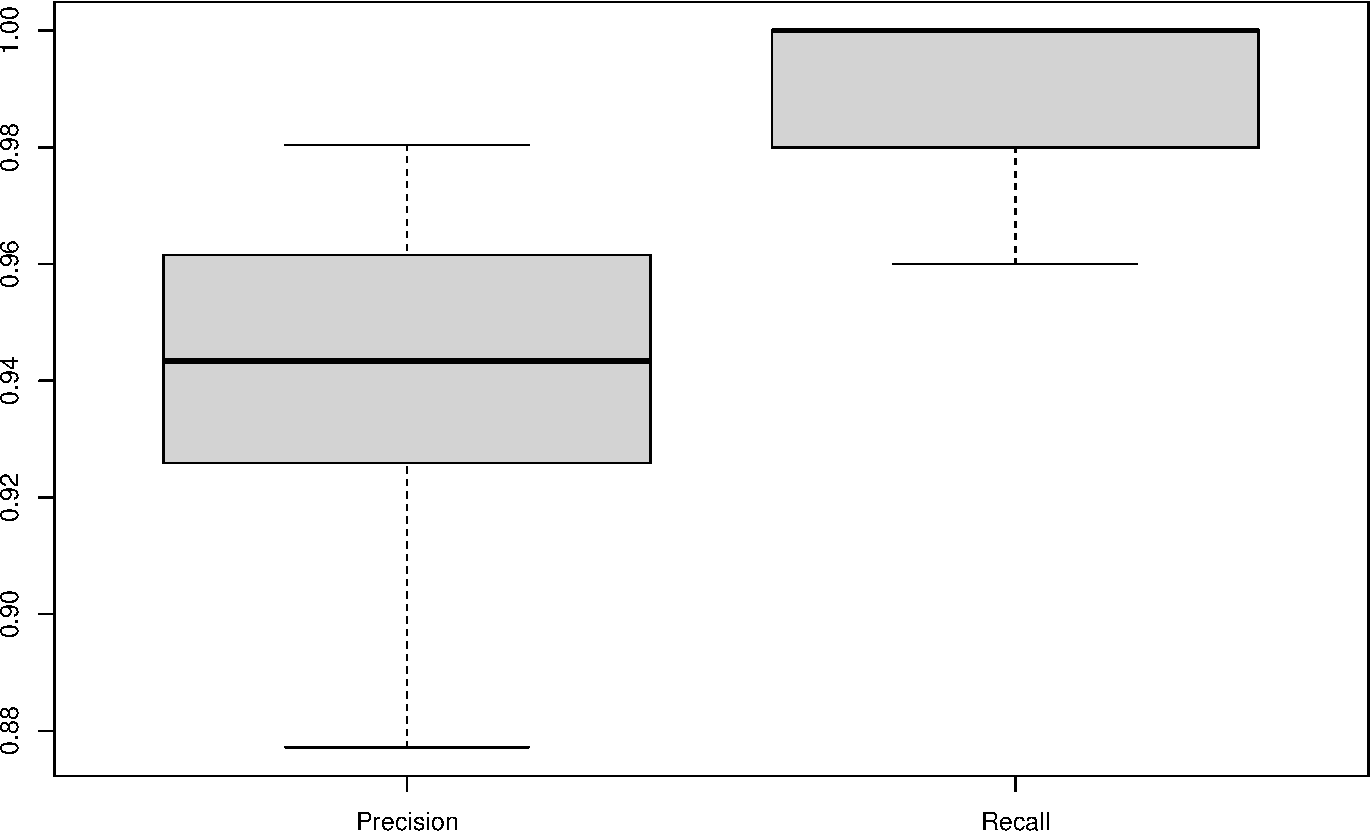
\includegraphics{bayesian-fellegi-sunter-vignette_files/figure-beamer/unnamed-chunk-12-1.pdf}

\end{frame}

\begin{frame}{Your Turn and Discussions}
\protect\hypertarget{your-turn-and-discussions}{}

\begin{itemize}
\item
  What other evaluation metrics would you look at?
\item
  Work on these either with a partner or in your free time?
\item
  What types of evaluations can we look at given the fact that this is
  an unsupervised problem?
\end{itemize}

\end{frame}

\begin{frame}{Your Turn and Discussions}
\protect\hypertarget{your-turn-and-discussions-1}{}

\begin{itemize}
\item
  You might think about how you would try and replicate the analysis
  that Sadinle did in his 2014 paper given this package.
\item
  Can you think of a simulation study to study the sensitivity of the
  method?
\item
  If you like this method, go read Sadinle (2017) and Sadinle (2018)!
\end{itemize}

\end{frame}

\end{document}
